\Titre{Postface}

\begin{Postface}

On peut dire, puisque de nos jours il faut toujours savoir tout caser et être en mesure de le faire avec brio, que «Le joueur de lyre» est un roman-blogue, un exercice Web 2.0, où un blogueur a bricolé une histoire en se connectant sur l’imaginaire, la connaissance, la culture, la générosité, le sens critique et le potentiel ludique de ses visiteurs-lecteurs-commentateurs. Voilà de quoi attirer l’attention des experts ès blogosphère et recevoir la médaille du mérite cybernétique. Mais dans le fond, «Le joueur de lyre» n’est qu’une simple aventure «littéraire» – souffrez que j’utilise ce terme - qui par-delà la mécanique Web, celle du portail Cyberpresse, de la masse d’abonnés, du logiciel WordPress et de l’infrastructure de télécommunications, puise dans une source éprouvée, celle du conte comme il s’en dit depuis la nuit des temps, depuis qu’il y a des enfants à aimer, à bercer, à faire glisser, tout doucement dans la dimension du rêve. Rappelez-vous, si vous avez eu ce bonheur, comment on raconte une histoire à un jeune enfant, le soir après le bain, après le petit pyjama, juste avant le dodo.

- Conte l’histoire du petit renard.

- Hum, celle où la poulette le chasse avec ses petites ailes en bataille ?

- Oui.

- OK. Hum ! Il était une fois, un vieux poulailler mal peinturé au milieu d’un enclos clôturé avec de la broche, où vivait une belle petite poule rousse…

- Non, pas rousse la poule, blanche.

- … où vivait une poulette toute blanche avec huit petits poussins tout jaunes…

- Non, elle n’avait pas de poussins, c’est sa maman qui en avait.

- OK c’est sa maman. Un jour, alors qu’elle grattait le sol avec sa petite patte à la recherche de nourriture en compagnie des petits poussins, elle vit se faufiler près du grillage, un petit renard …

- Tout maigre le petit renard … ehhhh, il faut dire renardeau …

- … un renardeau tout maigre qui n’avait rien mangé depuis trois jours.

- Il n’avait pas de maman, le renardeau ?

- Euh, elle était malade sa maman.

- Elle avait quoi ?

- Elle s’était fait mordre par un gros méchant chien très laid …

- Laid comment ?

- Pire que le chien de madame Rioux.

- Ouache… Je l’aime pas ton histoire.

- Elle ne pouvait pas aller chasser, la maman, et c’est le petit renard qui devait lui trouver de quoi se nourrir.

- Pauvre petit renard !

- Ouin ! Un jour, donc, la petite poule blanche aperçoit le petit renard et, les ailes abaissées, se met à caqueter très fort, comme pour dire : «Alerte, un renard, alerte !»

- Par où il pouvait passer, le petit renard, s’il y avait de la broche ?

- Les ratons laveurs avaient fait un trou dans le grillage et le fermier l’avait mal réparé.

- C’est méchant des ratons laveurs ?

- Non, pas vraiment.

- Ahhh.

- Donc, quand il a constaté qu’il avait été découvert, le petit renard s’est mis à pleurer. La petite poule blanche s’est approchée et lui a dit …»

Et ainsi de suite. C’est toujours ainsi. Vous avez une histoire dans la tête, c’est-à-dire un début, une fin et, entre les deux, un écheveau de faits et un début de collection de personnages. Au fur et à mesure que vous la dites, le bout de chou vous force à ajouter des détails, des séquences, des nuances, vous amène à revoir le ton, le débit, voire la morale et, surtout, vous permet de juger si vous êtes intéressant, ennuyeux ou assommant. C’est génial ! Il en est ainsi pour le roman-blogue. C’est un conte sain, simple et enrichissant, un exercice littéraire amusant, un jeu d’enfant, un jeu d’éternels enfants en quête d’émerveillement que nous serons tous jusqu’à la fin. C’est à l’opposé de ce qu’un auteur va fabriquer dans le silence, l’inquiétude et le doute, sans ces nutriments essentiels pour les uns, superflus ou redondants pour les autres, que sont l’interaction et la critique en direct.

Une autre considération à relever est la dimension feuilleton dans laquelle s’est drapé «Le Joueur de lyre». Inspiré à tort ou à raison par les grands écrivains du XIXe siècle, j’ai fait le pari de mettre un chapitre en ligne tous les vendredis matin et … je l’ai perdu. Effectivement, il m’a été impossible de le faire le 2 janvier 2009 en raison d’obligations familiales particulières au Nouvel An et de l’incontournable réalité d’un voyage à l’étranger. Reste qu’on parle de 20 semaines, de 19 chapitres, d’une quarantaine de dessins et de près de 132 000 mots (si je ne tiens pas compte de cette postface), soit une moyenne de 6 600 mots et deux dessins par semaine. Or il s’adonne que, durant cette période, mes vies personnelle et professionnelle ont exigé de très nombreux déplacements au Québec, en Ontario et, surtout, aux États-Unis. Tant et si bien que des chapitres entiers ont été écrits en auto, en avion, dans une chambre d’hôtel, dans une salle de presse, dans un sous-sol de Rimouski et même dans une tente de prospecteur, je vous jure ! J’entends d’ici la critique affirmer qu’à un tel rythme et dans de telles conditions, aucun roman digne de ce nom, ne pourra naître. À plus forte raison que l’auteur n’est pas un romancier, mais un journaliste. Un pisse-copie qui dessine de petits mickeys pour illustrer sa prose. Ça ne fait pas sérieux !

C’est là où, encore une fois, la techno vient déjouer ceux dont la pensée acquise est prodigieusement structurée, articulée, documentée, mais pleine d’inconnus par rapport au potentiel créateur des nouveaux outils.

Revoyons le processus que j’ai appliqué dans le cas de cette histoire de vieux Baby Boomers à qui les générations X, Y et Z font payer leurs vies dissolues.

Étape un : Récapitulation de la trame, articulation de la séquence du chapitre en cours, précisions des faits afin qu’ils soient plausibles, réflexions sur l’aspect humain des personnages mis en scènes dans ce chapitre. Cette étape a systématiquement été accomplie en discutant seul à seul avec ma conjointe, très souvent en auto.

Étape deux : Recherche dans les livres et sur le Web pour des explications généralement scientifiques et, parfois, pour des bouts de chanson dont j’ai oublié des paroles. Il y aura aussi des coups de téléphone, des échanges de courriel, des rencontres formelles afin que l’on m’explique ou me décortique un détail important.

Étape trois : Premier jet d’écriture et première version retravaillée et nettoyée de la majeure partie de ses fautes (merci Antidote !). En moyenne, j’ai eu besoin d’une vingtaine d’heures pour cette étape.

Étape quatre : Dessin de deux personnages et mise en ligne du chapitre illustré. Ajoutez ici un bon deux heures.

Étape cinq : Rétroaction grâce au système de commentaires offert par le logiciel WordPress. Dans les cinq ou six jours suivant la mise en ligne du chapitre, les lecteurs ont pu qualifier leur appréciation, suggérer des améliorations, critiquer un choix d’auteur, souligner et corriger des fautes et débattre d’un point soulevé. Jour après jour, j’ai pris connaissance de ces commentaires et, la plupart du temps, j’ai rapidement apporté les changements souhaités et les corrections qui s’imposaient. Parfois, cela m’a obligé de retourner en arrière dans des chapitres déjà publiés.»Vous maîtrisez avec perfection l’art de se r’virer sur un dix cennes», a écrit bibelot (pseudonyme d’une commentatrice devenue essentielle au sujet de laquelle je reviendrai plus loin). Ainsi, chaque chapitre se retrouve bonifié, épouillé, resserré, bref, réécrit. Certains connaîtront plus de dix versions, d’autres trois ou quatre. stvcc s’est dit impressionné par cette façon de faire. «Faut être humble en titi». En moyenne, j’ai eu besoin d’une dizaine d’heures pour cette étape, une étape qui, la plupart du temps, est venue se chamailler avec l’Étape trois.

Étape six : Une fois les dix-neuf chapitres commentés et retravaillés, je les ai polis d’une réécriture finale. Dans certains cas, p. ex. les chapitres 17 et 19, ce fut majeur. Dans d’autres, p. ex. les chapitres 5 et 13, ce fut mineur. C’est également à cette étape que j’ai rédigé la préface dans sa forme actuelle.

Étape sept : Rédaction du bilan que vous êtes en train de lire.

Ce que je viens de vous soutenir, c’est qu’en une semaine, période où j’ai quand même à assumer ma charge professionnelle de journaliste techno pour deux médias, un chapitre a été écrit de la plus belle façon que je le pouvais et publié sur mon blogue dans Technaute.ca, tandis qu’un autre a été scruté, corrigé, nuancé, bref, amélioré. Tout cela, dois-je le préciser, sans jamais utiliser une imprimante.

Ne serait-ce que par le temps impliqué, on est loin du fonctionnement traditionnel où l’auteur expédie par la poste (dans le cas d’imprimés) ou par courriel (document électronique) un chapitre à des amis ayant été embrigadés dans un «comité de lecture». Dans mon cas, je n’ai pas eu besoin d’une telle structure «amicale», puisque 56 abonnés à la Cyberpresse se sont portés «volontaires». C’est qu’au cœur du concept Web 2.0, il y a la notion de «communauté», et «Le joueur de lyre» a rapidement eu droit à la sienne, une communauté polie, drôle, généreuse et cultivée juste assez grande pour que je ne perde pas le nord.

\begin{floatingfigure}[r]{40mm}
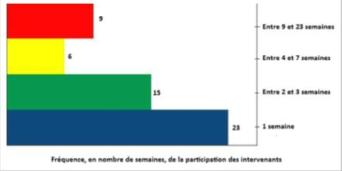
\includegraphics[height=60mm]{intro/postface/img/illustration2009021302.jpg}
\end{floatingfigure}

De ces 56 intervenants, 9 se sont manifestés sur au moins neuf semaines (dont 5 pendant plus de 15 semaines), 6 entre 4 et 7 semaines, 15, entre 2 et 3 semaines, 23 sur une seule semaine et un l’a fait au téléphone. Ici je ne calcule pas le nombre d’interventions où ces gens se sont exprimés dans la (ou les) semaine(s) où ils sont intervenus. Ce nombre a fluctué entre 10 (semaine du 26 décembre) et 102 (semaine du 19 septembre), sans qu’aucune tendance vers la baisse ou vers la hausse du nombre de commentaires ne se soit dégagée. On peut donc parler d’une communauté constituée d’une quinzaine de réguliers et d’une quarantaine de commentateurs plus discrets, des gens moins enclins à prodiguer leurs grains de sel.

Force m’est de signaler que sur les 56 participants, j’en connaissais sept :

    albel : mon beau-frère de Trois-Rivières. Fréquence : une semaine.
    alexanticosti : j’ai correspondu avec lui avant d’être à la Cyberpresse, mais je ne l’ai jamais rencontré. Fréquence : 15 semaines.
    jpmononk : un vieux copain depuis toujours. Fréquence : 3 semaines.
    laouise : une amie originaire de Rimouski. Fréquence : 13 semaines.
    madgab : ma grande fille bien-aimée qui est venue faire son tour sans m’avertir. Fréquence : une semaine.
    rejeanp : un vieux copain de longue date. Fréquence : aucune; il a utilisé le téléphone.
    snouppix : un vieux de la vieille que je connais depuis une quinzaine d’années. Fréquence : une semaine.

Ces gens, tous masqués d’un pseudonyme comme c’est la coutume sur Internet, des gens dont j’ignore l’identité (sauf ceux mentionnés ci-haut), bref de purs étrangers, m’ont fait le cadeau de nombreuses suggestions très utiles et sans lesquels la livraison du produit dans les délais prescrits n’aurait été possible.

Certains m’ont proposé des remaniements importants. Un bel exemple est cette suggestion qu’a publiée claude_c, le 5 septembre :

    «Bonjour Nelson, je vous propose, bien humblement, des coupures et aménagements, de façon à rendre le texte plus dynamique, et qu’on découvre les personnages plus rapidement. Certaines descriptions m’ont paru, à ce stade du récit, superflues. Mais il n’est pas dit que vous ne devriez pas les conserver pour la suite, au contraire. Vous en faites ce que vous voulez.»

Et là, le gars m’a copié-collé tout mon chapitre UN de la façon où lui l’avait redécoupé. Comme l’amélioration était majeure, je me suis empressé de l’accaparer et de faire les changements nécessaires.

D’autres ont pointé sur des passages qui mériteraient d’être un peu mieux tartinés. C’est le cas de cette suggestion de marcofsky qui est apparue le 2 novembre.

    «Le chapitre précédent annonçait un pivot dans l’histoire et on le sentait bien. Les événements de ce chapitre confirment cela, mais je trouve que l’intensité y fait un peu défaut. Par exemple, le dépucelage de Timothée: c’est un moment important, surtout que ça arrive à 43 ans ! N’y aurait-il pas lieu de “beurrer un peu plus épais” ? Mais surtout, de faire sentir au lecteur que, pour Timothée, cela a changé quelque chose. Idem pour la scène où on présente la lettre - je ne sens pas la “gravité” du moment, ni la surprise de Timothée ou celle de son père. Mais remarquez, c’est très subjectif ce que je dis, ce n’est qu’une impression.»

Et on m’a suggéré des réécritures. Par exemple ce paragraphe que m’a envoyé suzkinne, le 22 janvier, à la suite de commentaires sur ma nouvelle préface, paragraphe que je me suis dépêché d’aller coller en lieu et place du mien :

    «Il arrive quoi dans un sous-sol démoralisant, anémiant et sale, lorsque des gens jusque-là prostrés, cloîtrés et gommés des registres, se mettent à vivre toute une gamme de sentiments humains, partant de vieilles blessures cachées bien creux qui s’ouvrent, passant par des décennies de non-dit, de colère refoulée et d’ambitions détruites, finissant dans les larmes, le sourire et le bonheur ?»

Quelle chance j’ai eue, allez-vous dire. Attendez, il y a encore mieux. À plusieurs reprises, on m’a gratifié d’ajouts très intéressants dont certains ont contribué grandement à améliorer la qualité de mon histoire. C’est le cas de madgab qui, dès le chapitre 1, a surgi en ligne avec l’idée de créer un personnage canin, une sorte de chien hargneux et laid qui ajouterait à l’ordinaire des deux vieux illégaux enfermés dans leur sous-sol. Bibelot y est allé d’un prénom, Gazou, et d’un exemple de dialogue entre la vieillarde et son animal. Enfin, bernardprince a proposé un collier GPS qui permettrait au cabot de pouvoir faire sa promenade quotidienne sans avoir besoin d’humain ou de laisse. Quand on sait le rôle qu’a eu Gazou dans cette histoire, on ne peut que s’en féliciter.

C’est aussi le cas de dennis_dubeau qui a pensé à une pilule pour en finir, question de ne pas connaître le sort qui incombe aux vieux tel que décrit au chapitre 2. Encore une fois, Bibelot a fait du pouce et a suggéré un nom pour cet expédient, la «pilule du bonheur». C’est ce qui m’a amener à retravailler un rôle secondaire pour en faire quelque chose de beaucoup plus important, celui de l’ineffable Robespierre Alcide. Plus tard, le même dennis_dubeau a lancé l’idée de recourir au sabotage de la Saguewanish du chef de section Timothée Tardif. D’où le personnage du bonhomme Jean.

Et que dire d’albella qui, inopinément, m’a proposé une abomination sordide, soit un procédé de culture hormonale à partir de semi-cadavres. Cela a donné lieu à la naissance du sinistre docteur Bellavance, lequel, comme vous le savez maintenant, a fini par devenir gentil et attachant et s’est avéré très utile pour bien ficeler l’intrigue et le dénouement.

Autre bonne idée, alain_from_west a découvert une façon d’expliquer les pannes incessantes du système informatique utilisé au CRG-BSL. Selon lui, on aurait pu avoir recours à des «puces tatouées» rendant problématique l’utilisation de logiciels libres. Grâce à cette idée, il m’a fallu développer un personnage appelé Pierre Asselin, un vieil ingénieur logiciel quasi aveugle gardé dans une salle pour personnes en perte d’autonomie.

Pour sa part, suzkinne a fait deux interventions remarquées. Elle a commencé par nous produire une recette sérieuse du manger mou servi aux bénéficiaires, d’où l’appellation subséquente de Nutrisuz. Ensuite, elle nous a expliqué médicalement comment et pourquoi Marie Rioux était tombée malade, ce qui avait obligé Timothée à quérir l’aide du docteur Gagnon.

Parlant médecine, rejeanp, détenteur de je ne sais trop combien de diplômes universitaires en science, m’a corrigé le scénario médical de la mort du vieil anarchiste Robert Gagnon, alias Dart Vader. Commentateur occasionnel sur Technaute, il a préféré me téléphoner ses explications avant que je ne publie le chapitre en question.

Enfin, l’inénarrable flipper_21, grand praticien du calembour extrême, a suggéré d’utiliser le pseudonyme des contributeurs-commentateurs pour offrir des patronymes aux personnages secondaires de l’histoire. Sous un concert d’approbation, j’ai donné suite à cette idée dont voici le résultat.

    alain_from_west : Al Fromwest, partenaire informaticien de Pierre Asselin
    albella : le docteur Christian Bellavance, fermier hormonal qui n’avait jamais vu New York
    alexanticosti : Alessandro Costi, malfaiteur montréalais
    bernardprince : marque du collier GPS pour chiens solitaires
    bibelot : la bibliothécaire à sa retraite Bea Bellow
    bluesly et papynut : les frères Côtés, alias les horribles Papyblues
    claude_c : le jeune idéaliste Claude Sey
    dennis_dubeau : le chef des Verts, Thierry-Ian Dennis-Dubeau, alias Ti-Dédé
    flipper_21 : Phillipe Flipper Dauphin, le méchant directeur des communications
    jakeleblanc : le fonctionnaire économiste du Comité de déontologie Jacques Leblanc
    jpmononk : le représentant des bénéficiaires au Comité de déontologie, Jipé Gendron, alias Tit-mononk
    laouise : Louise Lavoie, responsable logistique au CRG-BSL
    marcofsky : Vlado Marcovsky, directeur de l’informatique au CRG-BSL
    rejeanp : le docteur Prévost, médecin légiste
    stvcc : joueur de cartes bègue appelé Steve Cécé en raison de son handicap
    suzkinne : Anton Suzkinne, inventeur du manger mou distribué par Monsanto sous le nom de Nutrisuz
    toogreen : l’agent de sécurité tropecolo
    ttc1 : L’agent de procuration Thomas Tremblay-Seyun, dans l’histoire des sacs de colostomie

D’ailleurs, voici la réaction de ce dernier commentateur en découvrant qu’il a inspiré un personnage. Très amusant !

    «Han ? Quoi ? Comment ? Moi ? “ttc1, l’agent de procuration Thomas Tremblay-Seyun (…)” ? C’est moi ça ? Woahhhh ! J’en suis toute chose. Non mais, m’as-tu me les taper les bretelles devant la galerie ! J’ai inspiré un personnage du premier roman-blogue de l’histoire québécoise (…). Je fais parti de la révolution Web 2.0 ! Whouhou ! C’est Warhol qui a dit que tout le monde avait son 15 minutes de gloire ? Je viens de vivre le mien. Merci Nelson !».

Mais toutes les suggestions n’ont pas été acceptées. La plus évidente est celle de prorats qui, comme l’indique son pseudonyme, voulait que j’ajoute des rats dans la description du CRG-BSL. Ouache ! Autre exemple, bluesly aurait aimé que mes personnages soient nantis d’implants électroniques sous-cutanés. Cette techno ne m’apparaissant pas comme pouvant être dominante dans 25 ans d’ici au point d’en faire bénéficier les vieillards, je ne l’ai pas retenue. Mais peut-être ai-je eu tort.

Et ce n’est pas tout. Qu’y a-t-il de plus désagréable à la lecture d’un roman, que de découvrir une erreur de fait. Par exemple, écrire que la violoncelliste Marie Rioux a joué pour l’Orchestre métropolitain de Montréal dans les années 70 alors que l’ensemble a été fondé au début des années 80. Ou aller visiter une dame dans son condo quand, deux chapitres plus tôt, on l’a fait vivre chez ses parents. Ou cacher un détail important à quelqu’un oubliant qu’on le lui a révélé trois chapitres en arrière. Ou être complètement à côté de la coche avec des horaires et des durées de trajet en autocar. Ou avoir camouflé des pilules du bonheur dans une boulette de papier aluminium alors qu’il y a des détecteurs aux portes du Centre gérontologique. Et ainsi de suite. À elle seule, la redoutable bibelot a débusqué huit de ces erreurs et suzkinne, deux. De quoi frémir !

Quelques-uns ont même accompli des tâches parfois fastidieuses, sans jamais demander quoi que ce soit. Comme ça ! Bénévolement ! Pour le plaisir ! La plus évidente et adulée de ces tâches est évidemment celle de bibelot qui, chapitre après chapitre, a tout récuré, sondé, soupesé, questionné et, d’un crayon rouge sang, corrigé. D’une semaine à l’autre, elle a imposé son autorité et a fait pâlir d’envie les linguistes et informaticiens à l’origine de la version d’Antidote que j’utilise religieusement. Étant personnellement victime d’une éducation bilingue, j’ai dû, en fin d’adolescence, réapprendre à écrire le français et … il est resté des traces. En plus, j’ai les doigts pleins de pouces et je tape à la diable. Bref, comme bien du monde, je fais des fautes. Parfois des gênantes. Des misères que je ne vois pas. J’ai beau comprendre «que je ne vois pas», en réalité c’est «que le de vois pas» qui est couché sur la page et je ne remarque rien. D’où Antidote ! Malgré cela, bibelot découvre de nouvelles «cidores». Voici ce qu’elle en dit:

    «Pourquoi je prends la peine de lire avec attention ? Par pur plaisir ! Depuis ma tendre enfance, je dévore tout ce qui se lit, même la boîte de céréales du déjeuner, sans blague. Votre roman-blogue me captive au plus haut point. Et traquer des cidores tient mon esprit en alerte.»

Et quand ce n’est elle, c’est Alexanticosti, suzkinne, flipper_21 et d’autres, dont laouise. «Cidores» ? C’est un acronyme de mon cru signifiant «coquille involontaire dont on regrette l’existence» (ce que marcofsky appelle «tapsus») qui, allez savoir pourquoi, s’est imposé dans les commentaires. De là sont venus les néologismes «cidoricide», «décidoriser» et «cidorigène».

Toujours à l’enseigne de l’aide désintéressée, il y a dennis_dubeau qui a écrit et enregistré un Blues inspiré par l’histoire de Marie Rioux qu’il a intitulé le «Blues de Gazou». Il y a également marcofsky qui, dès le départ, a offert ses services graphiques et qui a produit une galerie Web des personnages que j’ai dessinés. Quant à toogreen, l’homme de Shanghai, il a entretenu en ligne sur son propre blogue, une version PDF de mes chapitres.

Mais en plus de m’avoir fourni l’assistance nécessaire en raison du train d’enfer imposé par le mode feuilleton, ces gens anonymes m’ont fortement encouragé, pour parler en euphémisme. Ils m’ont permis de sentir, eux cette infime minorité d’internautes qui commentent en ligne, qu’il y avait du monde ici et là pouvant aimer ce que je faisais. C’est ce qui explique, chaque semaine, quand le doute venait frapper à ma porte, que je me raccrochais à eux et je continuais. Voici quelques exemples :

    «Ces personnages que vous avez su rendre attachants sont désormais ancrés dans mon univers imaginaire.» (bibelot)

    «J’étais tellement absorbé par la lecture qu’il n’y avait plus d’écran, plus de souris, plus de Technaute, rien. Rien que Timothée et cie.» (bluesly)

    «Personne ne pense plus à modifier l’histoire; on la suit comme du bonbon.» (dennis_dubeau)

    «Que les membres de mon entourage se le tiennent pour dit : ils vont découvrir un nouvel auteur au cours des prochains mois !» (flipper_21)

    «Cette belle histoire qui se termine ce soir, malheureusement (…) m’a donnée le goût de me remettre à … Lyre.» (jakeleblanc)

    «C’est déjanté, délirant et, en même temps, il y a de l’espoir. Les dessins sont extra, rien ne manque !» (laouise)

    «Merci pour ce beau roman sur lequel je suis tombé par hasard et que je me suis empressé de partager avec des amis dès ma lecture du premier chapitre.» (lewebiste)

    «Bon, parlons Art ! Parce que là, on y est ! Et pourquoi ? Parce que le conteur est maintenant à l’aise avec son récit et ses personnages. À l’aise également avec le rythme imposé soit un chapitre par semaine (…). Comme le musicien, c’est maintenant la mélodie qui l’anime et il ne pense plus à ses doigts, même s’ils sont occupés à jouer un solo d’enfer sur la guitare ! Le côté technique étant maîtrisé - et oublié - le talent peut maintenant être transcendé, tout bonnement par le plaisir ! Parce que c’est ce qu’on sent le plus dans ce chapitre, l’auteur a eu du plaisir à l’écrire. Et ça nous procure un plaisir unique à nous qui le lisons: ce n’est plus une question de style ou de genre, ou encore de pirouettes ou de bons mots, ça devient homogène et on le reconnaît : C’est le plaisir de lire du Dumais ! Merci, Nelson !» (marcofsky)

    «Quant à l’émotion qui se dégage de ce chapitre, j’en suis encore un peu gaga après une seconde lecture.» (papynut)

    «J’ai vraiment aimé l’histoire. Même que, pour mon cours de français, j’ai fait un exposé oral sur votre roman.» (ph.mongeau)

    «Si j’avais le roman en main, je ne pourrais interrompre ma lecture, je crois que le lirais tout d’une traite.» (suzkinne)

    «J’ai toujours hâte de lire la suite chaque semaine. Merci de prendre le temps de l’imaginer et de l’écrire.» (technaute.spamfree)

    «D’un chapitre à l’autre on ne peut prévoir la suite, c’est rebondissement sur rebondissement. Ça pourrait devenir très mélangeant et décousu, mais non, malgré tous ces intrigues et revirements, cette toile d’araignée se tient solidement sur ses ancrages et on suit le fil d’un chapitre à l’autre. (…) Les personnages sont vivants, crédibles et attachants.» (ttc1)

Si les commentateurs ont fait preuve d’autant de gentillesse, ils ne se sont pas privés d’amener des critiques pour autant, ce qu’ils ont toujours fait avec bonhommie, tact et délicatesse. Voici quelques exemples:

    «Fascinant! La Sociologie-Fiction a maintenant un nouveau chantre attitré: Nelson! Mais je ne suis pas aussi pessimiste. J’ai de bonnes raisons de croire que Nelson pousse le bouchon un peu loin lorsqu’il invente des chambres à gaz pour “réduire les coûts”. La tendance actuelle (ex. AQDMD) est plutôt vers plus de contrôle du “bénéficiaire” sur la date de sa mort plutôt que moins. Aussi, Nelson élimine un peu vite une autre tendance lourde, celle-là: la continuation du travail après l’âge canonique de la retraite, au moins pour ceux qui en retirent une certaine satisfaction. L’impact financier sera considérable. La vraie mort sociale c’est quand les autres n’ont plus besoin de nous.» (mvirard commentant le chapitre 2)

    «Comme je l’avais souligné dans le premier chapitre, je trouve que les informations incluses dans les blocs de descriptions ne sont pas assez livrées dans l’action. Dramatiser l’information. Et à mon avis, les descriptions contiennent trop de matières qui, pour l’instant, ne sont pas essentielles à la compréhension et au déroulement du récit. Si l’auteur tient absolument à les garder, pour alléger la lecture, il devrait les disséminer au fil du texte, au détour d’une réplique ou d’un paragraphe, pas nous les livrer en bloc. Et ne conserver que ce qui est nécessaire. Mais bon, c’est juste mon opinion, et ça vaut ce que ça vaut. (claude_c, à la suite du chapitre 2)

    «Ma seule critique sur le chapitre 19 serait que j’ai lu les 25 articles de l’entente en diagonale comme si de lire le contrat me sortait de l’histoire. La réplique de Romain à Turcotte est vraiment savoureuse… à partir de là, j’ai raccroché d’un seul trait jusqu’à la fin.» (bluesly déplorant la première présentation des articles imposés au ministre Turcotte)

    «Si cette œuvre se veut un véritable roman (…), alors mon ami Nelson, faut pas avoir peur d’y mettre tes tripes et de bonifier le document avec toute la gamme des émotions prévisibles dans ce type de situation. Personnellement je reste sur ma faim, j’ai l’impression de regarder un film sans dialogue et sans musique, C’est plutôt fade.» (alain_from_west sur une certaine sobriété qui avait caractérisé la première écriture du chapitre 7)

    «Les acronymes me distraient, car il me force à arrêter et à réfléchir sur ce qu’ils veulent dire… Ça ralentit le mouvement de l’histoire (…). Je préférerais les dénominations au long ou un synonyme, mais au long… (dennis_dubeau réagissant aux nombreux acronymes bureaucratiques que, dans un premier temps, j’avais parsemés ici et là pour faire encore plus Orwell)

    «Ce cinglé de Dart Vader m’a retourné l’estomac au point d’en avoir des convulsions (…). L’antithèse parfaite du Festin de Babette.» (bibelot au sujet de l’orgie alimentaire du chapitre 14)

    «Moi c’est ce qui a atterri dans le pare-brise qui me lève le cœur. J’en ai déjà eu un de même il y a plusieurs années ! Ouache ! Faut plus que j’y pense !» (lui répond laouise, référant à un geste de provocation posé par Robespierre dans le même chapitre.)

    «Ah ben prorats, t’aurais dû te taire ! Une chance que j’ai lu le chapitre avant la correction» (gemnoc qui réagit à la correction apportée à une répartie de la Maririou où j’avais oublié de la faire chuinter. C’est prorats qui avait signalé ce détail : «J’ai-tu manqué un chapitre ? La Maririou ne chuinte plus. Bonne nouvelle, ça va être plus facile à lire !»)

    «Un roman-blogue, cette invention que je n’ai toujours pas saisie !» (claude-henri, à la suite du chapitre 12)

    «Sincèrement, je n’ai jamais eu d’intérêt pour la Maririou. Je trouve que cela ne cadre vraiment pas avec le mandat de votre blogue. (…) Nous venons lire vos articles pour vos connaissances techniques et votre expérience et non pas pour lire votre passe-temps. Je vote pour la terminaison de la Maririou !» (lelecteuraverti amorçant un débat le 2 janvier; «La Maririou» était le titre de travail du Joueur de lyre.)

    «Je ne peux pas dire que le roman-blogue la Maririou est la partie que j’apprécie le plus de l’œuvre (de M. Dumais). Je suis un grand lecteur, je lis une vingtaine de romans par année, un par deux semaines environ, des polars principalement. (Mais) La Maririou, j’ai lâché après le premier chapitre. J’aime (…) le travail de M. Dumais lorsqu’il nous cause informatique (…).» wiiphone, le 2 janvier)

    «Je suis du même avis que lelecteuraverti. Je n’ai aucune idée de ce que fait cette nouvelle sur ce blogue qui n’est pas à sa base littéraire. Je me suis donc rapidement désintéressé de La Maririou. (…) J’avais, depuis un certain temps, tout simplement pris l’habitude de ne plus lire la chronique du vendredi. Maintenant que le sujet est sur le tapis, je sors du garde-robe avec mon opinion sur le sujet.» (nimzo, le 2 janvier)

    «Faut pas mal le prendre (mais) l’histoire ne m’intéresse pas vraiment. (…) Ce n’est pas pour moi. (Par contre), ce qui est fascinant pour moi, c’est l’interaction qu’elle provoque. (…) J’attends la suite des commentaires avec impatience. On ne voit pas ça souvent un auteur qui permet à ses lecteurs de le critiquer et de faire des révisions en direct.» (ianlambert, à la suite du chapitre 4)

Cette dernière remarque attire l’attention à juste titre sur l’interaction suscitée par le projet. Très rapidement, dès le chapitre un, les échanges entre commentateurs fusent de toutes parts. Le ton est, la plupart du temps, humoristique et des gens m’avouent les lire puisqu’ils sont … divertissants. Un trio se dégage assez vite de la mêlée, celui de dauphin_21, dennis_dubeau et alexantisosti. Certaines répliques sont totalement hors sujet, je les laisse quand même en ligne en raison se leur ton, de leur humour. Après tout, un roman-blogue, ce n’est pas une corvée canoniquement sérieuse, mais un divertissement collectif. Voici quelques exemples parmi tant d’autres tout aussi rigolotes:

    «Les Dumais, ça doit être fait forts en torrieu ; se placer ainsi sous la loupe (qui est la femelle du loup, tout le monde sait ça) d’une gang de téteux du dico, de la phrase juste, des régionalistes bien faits et du calembour à répétition (comme dans carabine à répétition). Je ne serai plus parfaitement objectif à la fin de cet exercice, alors je me garde trois ou quatre chum(e)s qui ont fréquenté Kerouac, Cavanna, Brétécher et Dard (pas l’épée là, le papa de Béru) à qui je me retiens à quatre sabots de refiler l’adresse de ce salon littéraire. Juste pour voir comment ça sera perçu, ce roman à multiples mains et une paire de nageoires… Entéka, ça ne devrait pas coûter trop cher en correction. J’ai aussi en réserve 3 amies (rien que des filles, tiens !) maniaques de la virgule bien placée, du parfait du subjonctif (plus difficile que l’imparfait du…) et amateuses de mots croisés, de l’Italie et de Falardeau (nobody’s perfect). Attends qu’elles passent sur ton texte mon Nelson, une horde de Bibelot. Ichhh. Allez mon Nelson, une double clef. Démolis-en quelques-uns. Tant pis si c’est des cousins. Fais-leur sortir le raisin. Faut que ça saigne.». (alexanticosti, le 28 octobre)

Le 14 novembre, un peu fatigué, j’ajoute à un commentaire de dennis-dubeau que j’aimerais pouvoir me consacrer à ce projet à temps plein et que j’en ai un peu marre, à ce jour, d’en avoir livré la moitié sur la route, dans des conditions peu propices à l’écriture. Ce à quoi ledit dubeau me répond :

    «Et qu’est-ce qui vous oblige à courir ? (…) Vous pourriez vous alléger la vie et rendre ce processus encore plus agréable pour vous en sautant une semaine sur deux ou en variant, un texte par mois ou par trois semaines. Ça vous laisserait respirer et nous, on aurait encore plus de fun créé par l’attente ! (…) Il n’est écrit nulle part que ceci doit se terminer CHAQUE vendredi !»

L’incisif alexanticosti lui rétorque alors :

    «Non non, laisse-le ramer le Dumais. C’est super bon ce qu’il écrit sur la run, s’il s’installe avec ses pantoufles, sa pipe et son chien roulé en boule à ses pieds il va nous pondre du Guy des Cars. Qu’il souffre l’Artiste. C’est pour notre plaisir …»

Puis, lui dont je m’étais inspiré pour le mafieux Alessandro Costi au chapitre 5, constate qu’un personnage de méchant, Philippe «Flipper» Dauphin, a été créé à partir du pseudonyme flipper_21 (le patronyme «Flipper» renvoie certains téléphiles au gentil mammifère marin). Voici un extrait de l’échange :

    «Éh que chu content de voir que le Flipper est un méchant. Il a que ce qu’il mérite, ce “ludoverbophile” (dauph) invétéré !» (alexanticosti)

    «À l’excroissance d’Anticosti : Hé-hé ! Je te ferai remarquer que ton personnage n’était guère plus gentil. En plus, y est mort ! Gniark gniark!» (Et flipper_21 signe “le Dauph’in tien vaut mieux que deux, tu l’auras.”)

    «J’aime mieux être mort en bobettes sur la route 138 que faire la démonstration de ma méchanceté dans un centre de vieux. En Sushi les dauphins ! Alessandro gontent de ce gui d’arrive.» (alexanticosti)

Comme Laouise, nouvelle venue, relève cet échange qui semble l’amuser, dennis_dubeau émet un soupir :

    «Bon, ça y est, on va encore passer pour une famille dysfonctionnelle. Content qu’elle ne remarque que les 2 pires ! »

La réaction ne tarde pas.

    «À la pilule dubeau neur (dennis_dubeau a en effet eu l’idée de la pilule): Famille dysfonctionnelle ? Nous ? Ben là ! C’est drôle que ce mot-là apparaisse quand tu réapparais. Je pense que Dumaître va bientôt nous passer l’étrangleur.» (flipper_21)

    «Met-z-en. Famille dysfonctionnelle, ça pointait full direct sur dubeau dubon ça mon homme ! Très perspicace Laouise. Elle a tout de suite “spotté” le celui qui est tout de traviole et reconnu que le machin aquatique et moi étions de très grande classe. Les deux pires. Pfff, tu ne sais donc pas que les jaloux ont un crapaud qui leur pousse dans l’estomac ? » (alexanticosti)

Reste que ce trio n’a pas le monopole de l’humour. Voici quelques exemples :

    «Nelson a écrit : “Merci pour votre intérêt à mes chiures de gomme !” Ouf ! Pendant un moment, j’ai cru qu’il avait inventé une nouvelle formule de politesse. Relisez sa phrase et omettez-le petit “à”. » (claude_c le 17 janvier)

    «Cidore ? (la discussion porte sur ces “cidores” que s’acharne à traquer bibelot) Personnellement, j’ai un faible pour le néologisme “Tapsus” dont voici la référence historique : “marcofsky, le Mercredi 20 Août 2008 : Je revendique la paternité du terme “tapsus”, soit un lapsus, mais au clavier - genre, on “tape su’ la mauvaise touche”… (à ne pas confondre avec “tape su ‘a yeule”, qui est autre chose complètement.)” »(vazimollo, le 6 décembre)

    «La la la la, lalalala la
    On m’appelle Bibelotine
    Parce que j’ai une drôle de mine
    Des cidores plein la figure
    C’est à cause de mes lectures

    Avec mon dico de poche
    Les cidores, je les caboche
    Et mon ami linuxien
    Ubuntuche, que j’aime bien
    La la la la, lalalala la» (bibelot, le 19 novembre, qui introduit ainsi son lot de correctifs à apporter)

    «Timothée – lyré» (alexpert qui réagit au fait que l’histoire ne s’appelle plus “La Maririou”, mais “Le joueur de lyre” et que, un mois auparavant, j’avais modifié le nom de “Timothée-Leary” (référence boomer aux drogues) en “Timothée-Milet” (référence musicale) pour des raisons particulières aux personnages de Marie Rioux.)

Le 2 janvier, j’ai proposé un jeu de fins alternatives. «Pendant deux ou trois vendredis, ai-je écrit, je pourrai vous publier une nouvelle version du chapitre final et vous voterez pour déterminer quelle sera la fin officielle». Masochisme ? Gâtisme ? Envie criante de faire durer le plaisir ? Qui sait ! Heureusement pour moi, l’idée ne lève pas vraiment. Seule laouise et, possiblement, guym, semblent en faveur. Marcofsky et alexanticosti l’écrasent vite fait - Masha’Allah ! - sous le poids de leur sagesse :

    «Vous nous avez démontré votre capacité à mener une intrigue tarabiscotée à souhait, (…), vous n’avez donc plus à le prouver en nous pondant une seconde ou troisième fin. (…) Ces finales alternatives dilueraient la qualité qu’une seule écriture réfléchie et concentrée (…) livrera à coup sûr. D’autre part, cette intrigue est le fruit de votre imagination, à plus forte raison son dénouement ! Le “jeu” auquel nous avons été conviés, sans avoir de règles établies, avait quand même cette limite, tacitement acceptée de tous, que cette histoire était la vôtre, tout comme les personnages (…). Bref, ce jeu des finales alternatives dénaturerait ce projet d’écriture en en changeant les règles à la toute fin. (…) Je ne jouerai pas ce jeu, ma pudeur artistique me l’interdit !» (markofsky)

    «Pour moi, il y aura une seule fin, celle que tu pondras. Qui forcément correspondra le mieux avec ce que tu as voulu raconter dans ce roman. Libre ensuite d’imaginer autant de fins alternatives que tu, ou qu’on voudra. Mais ce seront des variations.» (alexanticosti)

En résumé, il m’a été possible de raconter cette histoire et d’en publier une version pouvant être soumise à un éditeur, cela au travers mes contraintes professionnelles et en suivant un échéancier très serré, uniquement parce qu’une jolie brochette d’internautes anonymes s’est prêtée au jeu du roman-blogue; je suis convaincu que sans eux, je n’y serais pas arrivé. «Oui, mais il n’y en a eu que 56 qui se sont signalés dont une minorité qui s’est présentée sur une base régulière», me ferez-vous remarquer. «C’est vrai, mais heureusement qu’il n’y en a eu que 56», vous répondrai-je. C’est avec effroi que je songe à la masse de travail supplémentaire qu’auraient généré vingt, trente, cent, collaborateurs additionnels. Le produit final aurait-il été mieux ficelé ? Pas nécessairement, c’est à voir. Il faudrait peut-être tenter l’expérience et, croyez-moi, je n’envoie pas ici de message subtil aux bienveillantes autorités de la Cyberpresse.

Quant à cette version «pouvant être soumise à un éditeur», est-elle vraiment d’une qualité suffisante pour qu’on en fasse un bouquin, comme semblent le souhaiter bien des gens qui ont participé à cette aventure ? Honnêtement, j’ai déjà lu pire en provenance de maisons d’édition crédibles, mais j’ai aussi lu mieux. «Le joueur de lyre», ce sont quelque 137 000 mots pondus, assemblés, harmonisés et nettoyés en 20 semaines, quand on sait que de grands auteurs mettent parfois plusieurs années pour écrire un ouvrage, Michel Folco est un bon exemple. En revanche, il y en a d’autres, je pense à Amélie Nothomb et ses 25 000 mots annuels, qui présenteront une fréquence supérieure. Bien sûr, le temps n’a parfois rien à voir avec la qualité de l’œuvre quand le génie de l’auteur occupe toute la place. Mais moi qui ne suis ni Folco ni Nothomb, je suis un journaliste qui n’a de prétention que dans l’exercice de son métier, je me doute bien qu’un mois ou deux de plus auraient pu améliorer le produit. Claude_c a bien résumé cette situation en marge du chapitre 2. «Le talent, c’est 95% de transpiration et 5% d’inspiration; à chacun sa méthode et son désodorisant», a-t-il écrit.

En d’autres termes, «Le joueur de lyre» est une histoire comme il y en a bien d’autres, une histoire que j’ai voulue divertissante sans être idiote et que j’ai «montée», pardonnez-moi ce terme cinématographique, de façon à ce qu’elle puisse tirer son épingle du jeu dans un contexte où l’audiovisuel prend toute la place. «On ne lit pas ce roman, on le regarde, a commenté ttc1. L’imagerie mentale que cette lecture génère est phénoménale.» Quant à affirmer que «Le joueur de lyre» fait le poids dans l’hallucinante offre de produits artistiques d’expression française, j’en suis incapable n’étant pas outillé pour le savoir, à plus forte raison que j’ai éprouvé beaucoup de plaisir à en assumer le quotidien.

Merci à tous ceux qui ont bien voulu participer (leurs pseudonymes suivent ci-après en ordre alphabétique) ; je suis hautement impressionné par la qualité de leurs commentaires, lesquels on peut consulter en naviguant sous cette adresse chapiteau.

    alain_from_west
    albella
    Alexanticosti
    alexpert
    atouat
    Bernardprince
    bibelot
    bigsimbad
    bluesly
    christine63
    claude_c
    claude-henri
    dennis_dubeau
    Dragon68
    embryon
    ericdesh
    flem187
    flipper_21
    gemnoc
    gilas
    guym
    I.com
    ianlambert
    jakeleblanc
    jmv1
    jpmononk
    laouise
    lelecteuraverti
    lewebiste
    madgab
    marcofski
    marcximus
    mephistau
    mvirard
    nickoleterrible
    nimzo
    papynut
    paquind
    ph.mongeau
    phantoman
    plante_ca
    porfilio
    prorats
    rejeanp
    robertduquette
    Sabrina1
    snouppix
    stvcc
    suzkinne
    sythas
    technaute.spamfree
    toogreen
    trocupei
    ttc1
    vazimollo
    wiiphone

\end{Postface}